%!TEX encoding=UTF-8 Unicode
\chapter{Analyzing Fine Grained Memory Traces}

\gls{Tabarnac} traces contains two parts: informations about the data structures and the actual trace.
For small applications with a limited number of data structures, it is trivial to present the first kind of information.
The actual trace is spread over three dimensions: threads, pages and type of accesses however this last one can only take two values (read or write).
Therefore it is relatively easy to find a meaningful representation of this traces that can be easily understood by a human.
\gls{Moca} traces are way more generic.
Indeed, they contain the same meta data and the actual trace also provides informations about time and \gls{CPU} location.
These traces are spread over five dimensions: time, addresses, type of access, and \gls{CPU} location.
Furthermore some dimension can be seen from several point of view, for instance we can look either at the physical or virtual address space.
As we are not used to visualize things in more than three dimension, to analyze these traces, we must provide the user a way to navigate through different representations and easily find and focus on the important parts.

The contribution presented in this chapter consists in two different methods to analyze \gls{Moca} traces:
\begin{itemize}
    \item The first method relies on \gls{Framesoc}~\cite{Pagano14frameSoC}, an existing generic trace management tool, and more specifically one plugin called \gls{Ocelotl}~\cite{Dosimont14Ocelotl} that provide aggregated views of a trace.\\
        We have implemented an importer to analyze \gls{Moca} traces in \gls{Framesoc} that is distributed on Github under GPL License:\\
        \url{https://github.com/dbeniamine/framesoc\_importer\_moca}.\\
        \DB{Distribute properly moca importer}
        The proposed visualizations are presented in an Inria Research Report~\cite{Beniamine15Memory}.
    \item The second method relies on \gls{R}, it is an ongoing work, publicly available online:\DB{Make labbook public}
\end{itemize}

This chapter is organized as follows: first we present our analysis of \gls{Moca} traces with \gls{Framesoc} and \gls{Ocelotl} with an example and discuss the limits of this method in \sect{visu-first}.
Then we propose a second, more flexible approach base on \gls{R} in \sect{visu-second}.
Finally we present some perspective of work to improves these analysis and our conclusions in \sect{visu-cncl}.


\section{Interactive visualization of aggregated traces}
\label{sec:visu-first}

As \gls{Moca} traces are spread over five dimensions and as the address space of an application can be quite large, we need a way to navigate easily in the trace and highlight interesting parts.
Consequently, we are looking for a tool that have a model of the trace and the ability to spot anomalies.
While several generic trace manager tools such as \gls{HPCToolkit}~\cite{Adhianto10HPCTOOLKIT} are able to import generic traces, we decided to use \gls{Framesoc}~\cite{Pagano14frameSoC}.
This decision was mainly motivated by one of \gls{Framesoc} visualization tool, \gls{Ocelotl}~\cite{Dosimont14Ocelotl} that is designed specifically to aggregate similar parts of a trace and identify anomalies.

\subsection{FrameSoc and Ocelotl}

\gls{Framesoc} is a generic trace management, it provides importers to read traces from many different format.
From its point of view a trace consists on four sets:
\begin{enumerate}
    \item Some meta data on the trace, such as the name of the trace, the application traced, the number of \glspl{CPU} used, the \gls{OS} etc.
    \item A set of \emph{Event Producers}: which are entities able to produce some \emph{Events}.
        For classic performance traces the Event producers are the \glspl{CPU}.
    \item A set of \emph{Events}, \emph{Variables} and \emph{States}: for instance in a classic trace, a call to a \gls{MPI} function could be an event, and a \gls{CPU} could be in \emph{idle} state after a call to \texttt{MPI\_Receive}. Variables are used to represent events that have a specific values and last over time.
    \item A set of \emph{Links} that can be used to represent causality between events, variables and states.
\end{enumerate}

To analyze a trace from an unknown format in \gls{Framesoc}, we need to write an importer which is a relatively simple task.
Indeed \gls{Framesoc} is implemented as an Eclipse plugin, consequently an importer is a small piece of java code that read a trace file, create the sets described above and store them in a database, using \gls{Framesoc} \gls{API}.
The main difficulty of this task is to represent a trace with \gls{Framesoc} model.

\gls{Framesoc} provides several functionalities to explore a trace such as filtering events by type, name, focusing on a time frame, etc.
Additionally it has a multi view representation which means that several views of the trace can be opened at the same time and synchronized.
For instance a user can start inspecting a trace with a Gantt chart, focus on a small part and then look at a pie chart of the event distribution on this subset of the trace.
\gls{Framesoc} is optimized to make such analysis as smooth as possible.

\gls{Ocelotl}~\cite{Dosimont14Ocelotl} is an analysis tool for \gls{Framesoc}.
This tool is particularly interesting for us as it is provide an aggregated overview of a trace.
The idea behind \gls{Ocelotl} is that a trace with too much entities (events or event producers) is not understandable, consequently, it should be analyzed with a \emph{systemic approach}.
This means considering the whole trace as a system and finding a macroscopic representation of that system that contain an amount of information understandable by a human.
To do so, it uses an aggregation methodology proposed by Lamarache-Perrin~\cite{Lamarche_Perrin14Agregation} and adapted for trace analysis.
This methodology cuts the trace on small slices over the two dimensions time and space (event producers).
Then it consider each meaningful partition possible, benefiting from the structure on time and space to reduce the number of possibility.
For instance merging two slices that are not continuous over time is not allowed as it would not be meaningful.
In addition, it uses a parameter $p<[0,1]$ that controls the trade-off between information loss and data reduction and find the optimal partition for this parameters.
Once the first visualization is generated, \gls{Ocelotl} provide the ability to explore the trace (zoom, use \gls{Framesoc} filters \ldots) and change the $p$ parameter.
The usual workflow with \gls{Ocelotl} is starting with a high $p$, where the trace is mostly aggregated, zoom on anomalies or interesting parts and decreasing $p$ to understand more precisely what phenomena we are observing.

\begin{figure}[htb]
    \centering
    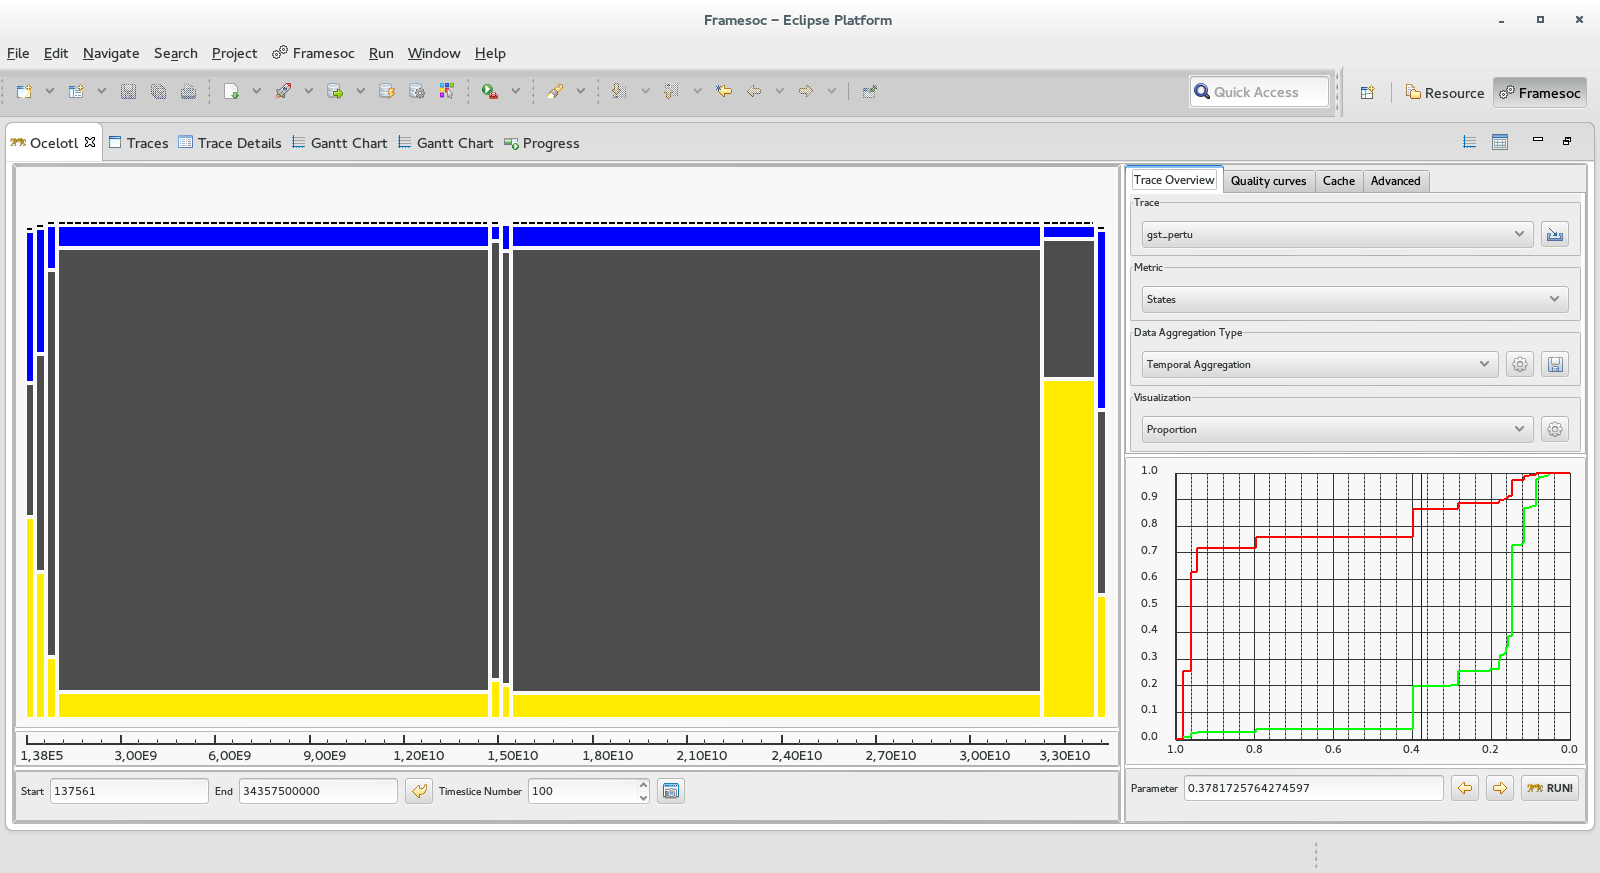
\includegraphics[width=\linewidth]{ocelotl}
    \caption[Screenshot of Ocelotl.]{
        Screenshot of Ocelotl highlighting an irregularity in a trace.\\
        Overview of the trace on the left, curves showing the impact of the $p$ parameters on the complexity of the trace on the bottom right.\\
        Image from~\cite{Dosimont14Ocelotl}.}
    \label{fig:ocelotl-overview}
\end{figure}

\fig{ocelotl-overview} is a screenshot of \gls{Ocelotl}, showing on the main pane an overview of an example trace, aggregated over the time.
On this overview we can see two huge aggregated blocks, in the middle, two smalls ones between them, and a few small blocks at the beginning and at the end of the execution.
Without knowing anything about the trace displayed, we can understand that their is an initialization and a finalization phase as they are not aggregated with the rest of the execution.
Moreover the main part of the execution is split in two, either their is a transition between two phases or a perturbation in the middle.
At this point the user could zoom in a subpart of the trace by selecting it, or change the parameter $p$ to disaggregate the visualization.
We can see a window on the bottom right corner showing curves about the  amount of information loss and data reduction for each possible value of $p$.
Under the curves, the current value of $p$ ($3.7$) is displayed.
It is possible to change it manually or directly click on the part of the curves that seems interesting.


\subsection{Trace Description}

As explained earlier, \gls{Moca} traces are spread on five dimensions while \gls{Framesoc} is designed for two dimensional traces (time and event producers).
Nevertheless we can use the \emph{event type} of \gls{Framesoc} to differentiate reads from writes.
Moreover, event producers are organized hierarchically, therefore we can represent two dimensions as one by using this hierarchy.
For instance if we consider that each thread is a root level event producer and embed the whole memory hierarchy, we can represent at the same time memory and threads.
Finally, as we cannot reorganize dynamically the hierarchy of event producers, another workaround consist in creating several traces with different event producer hierarchy.

We designed a \gls{Framesoc} importer for \gls{Moca} traces which produces three different \gls{Framesoc} traces.
The first one create an event hierarchy based on the virtual memory addresses.
The second one does the same thing for physical addresses.
Finally, in the third one, each thread is a root event producer and embed the whole memory hierarchy.

The more event producer there are, the more partitions \gls{Ocelotl} must consider to compute the aggregation.
Yet, \gls{Ocelotl} uses the structure of the event producer hierarchy to reduce the number of allowed partitions.
Consequently we can counterbalance the huge number of event producers by creating an artificial hierarchy in the memory.
We can build a meaningful hierarchy that also adds some semantic to the trace: to do so we create a virtual \emph{Memory Root} event producer that is the parent of every event producers.
Then the second level of event producers is composed of the stacks and data structures.
All the addresses that are not in these set, are merged if they are contiguous, creating chunks of continuous addresses which are also second level event producers.
Then each level is obtained by splitting the previous one on two or three parts, until we arrive at the page level.
The pages are the leaves of this virtual memory hierarchy.
We could divide the pages in cache lines and keep going until the address granularity, but this would generate way more event producer that what \gls{Ocelotl} is able to handle.

\begin{figure}[htb]
    \centering
    %!TEX encoding=UTF-8 Unicode
% Palette Dark2 3 colors
\definecolor{ColF}{HTML}{1B9E77}
\definecolor{ColV}{HTML}{D95F02}
\definecolor{ColM}{HTML}{7570B3}



\tikzset{
    % Args: BeginVal, EndVal, Size, label, Color
    pics/access/.style args={#1#2#3#4#5}{
        code={
            \draw[|-|,thick,#5] (0,0) node[pos=0,below=2pt,#5]{#1} -- (#3,0)
            node[pos=1,below=2pt,#5]{#2};
            \node[ColV][anchor=south] at (#3/2,0) {#4};
        }
    },
}
\tikzstyle{mybrace} = [decorate,decoration={brace, mirror,amplitude=1em},thick]

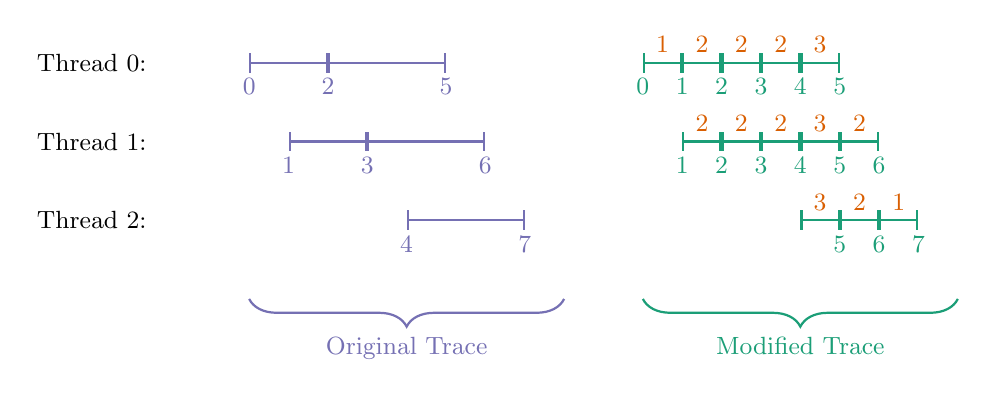
\begin{tikzpicture}[font=\small]
    \node at (-2,0) {Thread 0:};
    \node at (-2,-1) {Thread 1:};
    \node at (-2,-2) {Thread 2:};

    \draw[mybrace,ColM] (0,-3) -- (4,-3) node[pos=.5,below=1em] {Original Trace};
    \draw[mybrace,ColF] (5,-3) -- (9,-3) node[pos=.5,below=1em] {Modified Trace};

    % Moca trace
    \pic at (0,0)       {access={0}{2}{1}{}{ColM}};
    \pic at (1,0)       {access={ }{5}{1.5}{}{ColM}};

    \pic at (0.5,-1)    {access={1}{3}{1}{}{ColM}};
    \pic at (1.5,-1)    {access={ }{6}{1.5}{}{ColM}};

    \pic at (2,-2)      {access={4}{7}{1.5}{}{ColM}};

    % After parsing
    \pic at (5,0)       {access={0}{1}{.5}{1}{ColF}};
    \pic at (5.5,0)     {access={ }{2}{.5}{2}{ColF}};
    \pic at (6,0)       {access={ }{3}{.5}{2}{ColF}};
    \pic at (6.5,0)     {access={ }{4}{.5}{2}{ColF}};
    \pic at (7,0)       {access={ }{5}{.5}{3}{ColF}};

    \pic at (5.5,-1)    {access={1}{2}{.5}{2}{ColF}};
    \pic at (6,-1)      {access={ }{3}{.5}{2}{ColF}};
    \pic at (6.5,-1)    {access={ }{4}{.5}{2}{ColF}};
    \pic at (7,-1)      {access={ }{5}{.5}{3}{ColF}};
    \pic at (7.5,-1)    {access={ }{6}{.5}{2}{ColF}};

    \pic at (7,-2)      {access={ }{5}{.5}{3}{ColF}};
    \pic at (7.5,-2)    {access={ }{6}{.5}{2}{ColF}};
    \pic at (8,-2)      {access={ }{7}{.5}{1}{ColF}};
\end{tikzpicture}
% vim: et si sta lbr  sw=4 ts=4 spelllang=en_us

    \caption[Sharing detection on Moca traces.]{
        Sharing detection on a Moca trace, where three threads accesses the same page over the time.\\
        Each access is represented as an interval of time.\\
        Original trace on the left, accesses are not annotated, timelines are not synchronized.\\
        Modified trace on the right: timeline are synchronized and accesses are annotated with the number of thread involved in the sharing.
    }
    \label{fig:sharing-detection}
\end{figure}

To keep the thread information in the two first traces, we pre process \gls{Moca} traces to mark each access as shared or private.
In \gls{Moca} traces, each access is timestamped by the beginning and end of the chunk to which it belongs.
Furthermore, \gls{Moca} traces are \emph{complete} at the page granularity.
Hence, we consider that an access is shared if and only if two threads accessed the same page during intersecting time lapse.
To compute this sharing, we retrieve the list of accesses for each page.
We consider that an access is an interval of time during which the page is used.
Hence we only need to compute overlapping intervals.
\fig{sharing-detection} show how we transform \gls{Moca} traces to add sharing information.

Each access is represented by a variable, whose value is the number of threads involved in the access.
Our traces have four types of accesses: \texttt{PrivateRead}, \texttt{PrivateWrite}, \texttt{SharedRead} and \texttt{SharedWrite}.
Finally, the \gls{CPU} on which the access occurred is stored as an event parameter.

\subsection{Example}

\begin{algorithm}
    \caption{Naïve parallel matrix multiplication.}
    \label{alg:mat-par}
    \begin{algorithmic}
        \For{i=0; i<sz; i++}
            \For{j=myid(); j<sz; j+=NbThreads()}
                \For{k=0; k<sz; k++}
                    \State Res[i][j]+=A[i][k]*B[k][j]
                \EndFor
            \EndFor
        \EndFor
    \end{algorithmic}
\end{algorithm}

To illustrate these visualizations we implemented an extremely naïve parallel matrix multiplication.
In this example, a first thread does the whole initialization, then create two threads that will do the actual computations.
Furthermore, we split the work between the threads in a round robin way, the first thread computes all even columns and the second does the odd ones as described in \alg{mat-par}.

\begin{figure}[htb]
    \centering
    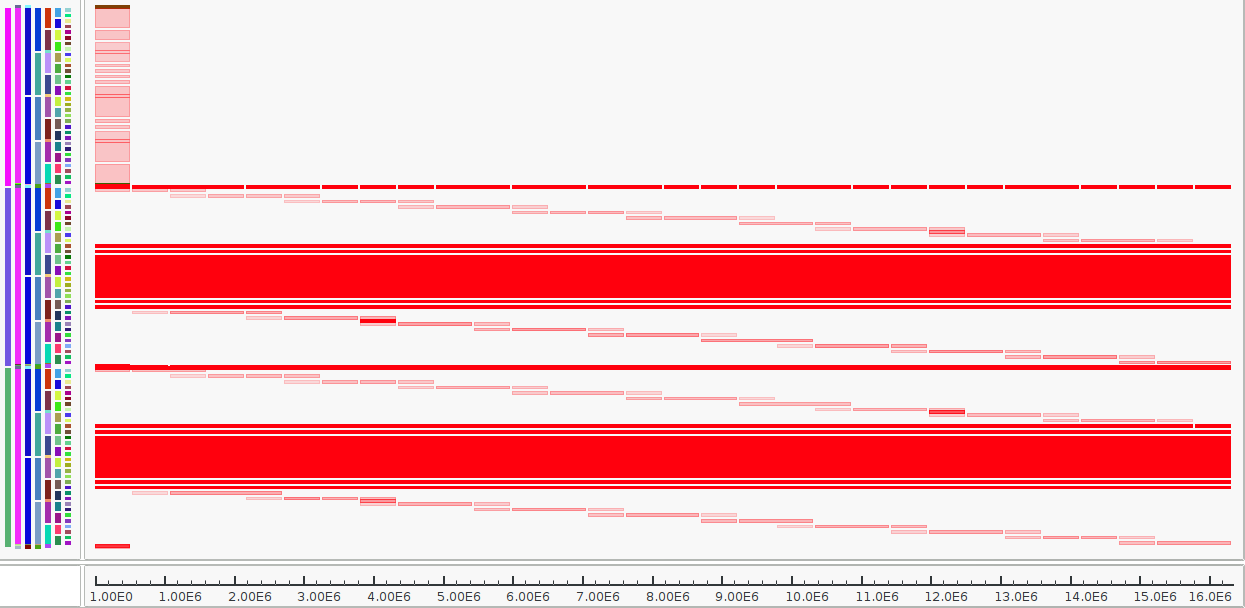
\includegraphics[width=\textwidth]{Moca-RR/multModuloThreadView.png}
    \caption{Memory-gantt view of the naïve parallel matrix multiplication.}
    \label{fig:ocelotl-th0}
\end{figure}

\fig{ocelotl-th0} is a screenshot of \gls{Ocelotl} visualization of \gls{Moca} trace, where the hierarchy starts by the threads of the application.
We can see the hierarchy on the Y-axis, starting with the three threads, each embedding the whole memory hierarchy.
The X-axis represent temporal evolution.
We call this view Memory-gantt.

From this view, we see clearly the master slave behavior of the threads.
While the two slave threads have a similar memory access pattern, the master thread on the top of \fig{ocelotl-th0}, does all its accesses at the beginning of the execution.
Moreover it seems to access all the memory at once.
We can also see that it does less access at a time as the blocks are lighter.
From this picture, we can clearly identify two phases:
\begin{enumerate}
    \item The three threads seem to use the memory, it is the initialization phase.
    \item Only two threads are awake, they follow the same access pattern: it
        is the computational phase.
\end{enumerate}

\begin{figure}[htb]
    \centering
    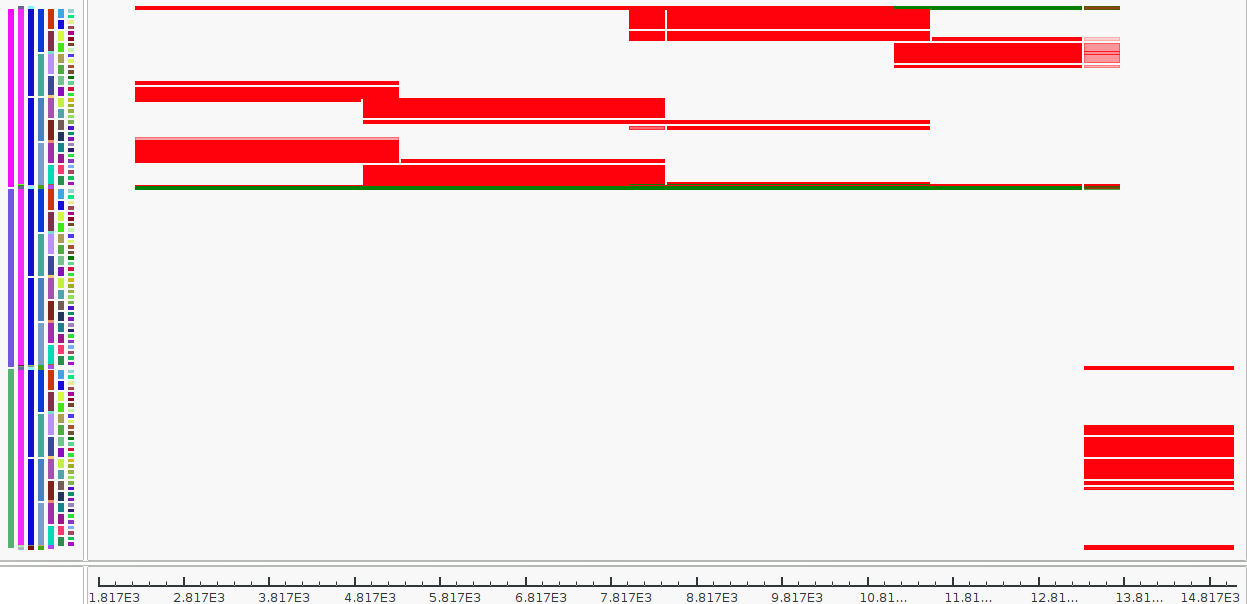
\includegraphics[width=\textwidth]{Moca-RR/multModuloThreadViewInit.png}
    \caption{Memory-gantt view of the naïve parallel matrix multiplication ,
    initialisation}
    \label{fig:ocelotl-th1}
\end{figure}

Now let's zoom on the initialisation step.
The result is shown in \fig{ocelotl-th1}.
We can clearly see that, contrary to what we thought on the last picture, during the initialisation phase, only the master thread is working.
We can identify a three diagonal patterns happening at the same time, it correspond to the matrix initialisation.
Moreover we see a few green access, while all the other are reds.
Here a red access mean that it is on a page used by several threads, while green is for private data.
Therefore we can see that the master thread also access to some private data.
Among these data, we can find a pid array used to wait the end of the slave threads.

\begin{figure}[htb]
    \centering
    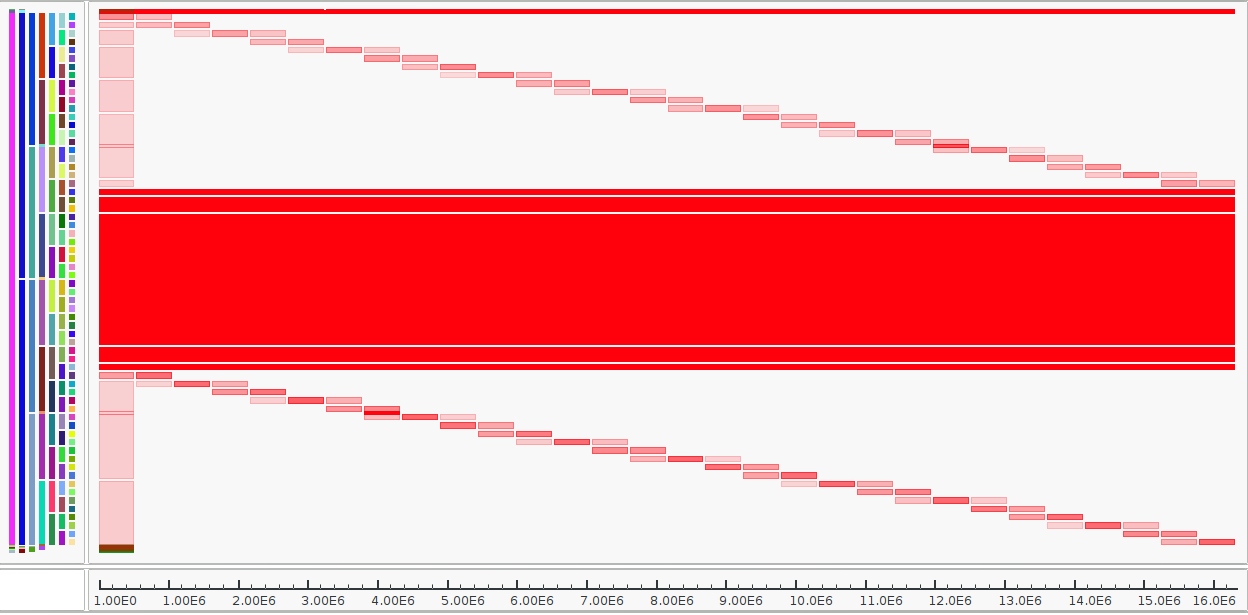
\includegraphics[width=\textwidth]{Moca-RR/multModuloCartoView.png}
    \caption{Cartography view of the naïve parallel matrix multiplication.}
    \label{fig:ocelotl-carto0}
\end{figure}

The cartography view (trace without the threads in the hierarchy) of this initialisation phase, is almost identical except that we won't be able to know which thread is responsible for the accesses.
However the global cartography view shown in \fig{ocelotl-carto0} gives more information.
In addition to the two execution phases, we can clearly identify three memory structures with different access patterns.
Those structures correspond to the matrices.
For the first and the third, we can see a regular diagonal access pattern which means that the matrix are accessed linearly, which is an efficient memory pattern.

\begin{figure}[htb]
    \centering
    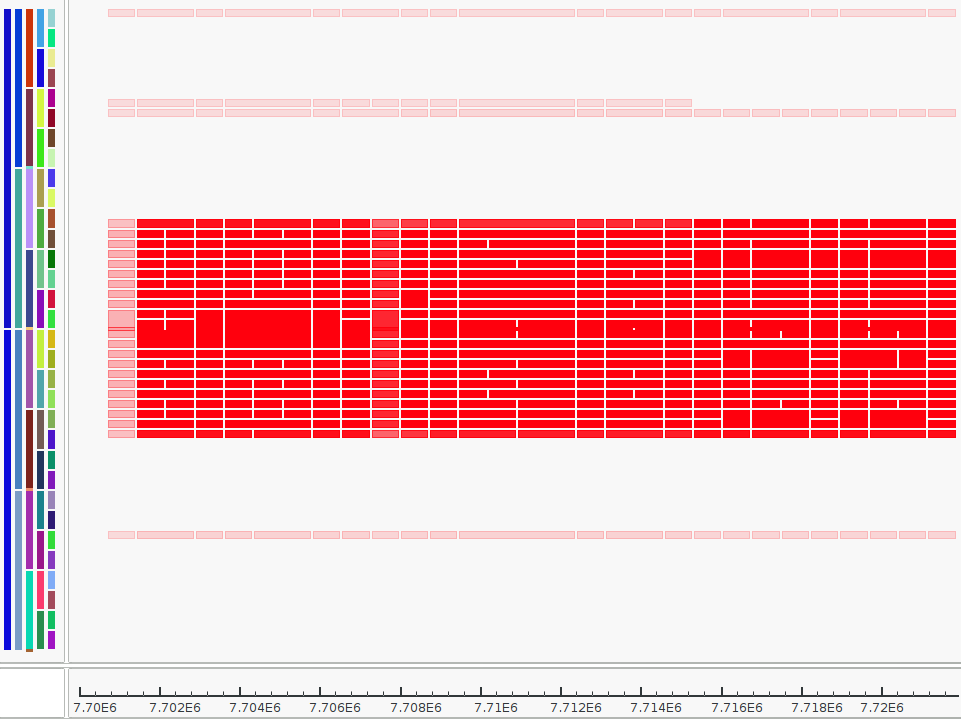
\includegraphics[width=\textwidth]{Moca-RR/multModuloCartoViewMiddle2.png}
    \caption{Cartography view of the naïve parallel matrix multiplication, computing phase.}
    \label{fig:ocelotl-Carto2}
\end{figure}

By focusing on the middle of the execution and setting the aggregation to zero, we obtain the \fig{ocelotl-Carto2}.
We can't identify a clear pattern on the middle matrix, however, we see that at each time slots we access a slightly different part of the matrix (the lighter a block is, the less access it contains).
The access on this matrix seems  dense and not designed to fit in a cache.
This density of accesses is coherent with the behavior described in \alg{mat-par}
Indeed, each thread goes through all the matrix B while working on only one line of A.
Moreover the two threads works on two different columns at the same time, while the work on the same lines of A and Res.
Due to the representation of 2D matrix in \texttt{C}, each access on B is separated from $sz$ doubles.
Hence \gls{Ocelotl} groups almost everything in a huge chunks of access on all the matrices.
%To improve this application, we should try to work on small blocks of B.
%This is indeed the strategy used to compute efficient matrix multiplication.

\subsection{Discussion}

Although we were able to visualize all the inefficient patterns in the example described previously, we were not completely convinced of the visualization based on \gls{Ocelotl}.
Indeed, the first limitation comes from the fact that \gls{Framesoc} trace description is quite static and does not permit to change the event producers.
As a result we had to generate three traces (virtual addresses, physical addresses and by threads) to provide different visualizations.
This means that if we spot an interesting pattern in a visualization and want to look at it from another point of view, we need to reload the whole trace and  which breaks the flow of trace analysis.
Indeed \gls{Ocelotl} initial computations are slow as it requires to compare all possible partitions.
Additionally, by doing so we loose all filtering and zoom done on the previous trace.

\DB{Reformuler:}
Another limit of this approach is that it is hard to identify (name) the data structure.
Furthermore selecting only a set of data structure is slow as \gls{Framesoc} is not designed for handling as much event producers as we have with memory traces.
Finally meta data about there size or number of accesses are impossible to visualize.

To conclude, these visualization are interesting and enables identification classic mistakes.
Yet it seems that in the end \gls{Ocelotl} tool is no well suited for memory traces.
Therefore we should try a more dynamic approach that permit to change the point of view easily.

\section{Programmatic exploration}
\label{sec:visu-second}

The main drawback of using a generic visualization tool for analyzing \gls{Moca} traces come from the difficulty to switch the perspective from which we visualize the data.
This limitation comes from the static representation of the trace as a two dimensional entity.
Hence, a more programmatic approach may enable to work closer to the data and ease this point of view switch.
In \gls{R}, data are usually stored in huge dataframes, each row of a dataframe represent one observation and each column give the value of a parameter or a measure for this observation.
While this representation has a significant memory footprint, it ease switching point of view, as the same dataframe can represent several measures.
For these reason, we analyzed several traces with \gls{R}.
For more reproducibility, we store the evolution of our work in an \gls{Org-mode} labbook, as described in~\cite[Chapter~4, p~54]{Stanisic15Reproducible}, and available online at \url{TODO}.

While this approach is extremely flexible, it is not user friendly.
Indeed it requires to know how to write efficient \gls{R} code, how to use \gls{Org-mode} and Emacs and to read the labbook before doing an analysis.
Anyway, after a few analysis we obtained a basic procedure to analyze traces (parsing, transforming data, showing some generic visualization) from which we can adapt each step to the trace.
For instance we might want to ignore some parts of the trace very soon to focus on some data structures, or after analyzing one plot we might think of another representation of data that might be meaningful in this case.

\subsection{Design}

Our analysis converged very quickly to a classical yet adaptable analysis pipeline:
\begin{enumerate}
    \item Parsing: reading \gls{Moca} traces (to which we have applied the sharing detection written for \gls{Framesoc} and depicted in \fig{sharing-detection})
        and representing the data in a \gls{R} friendly way.
        At the end of this step, we have two dataframes, the main one contains all the accesses, and the other one the list of data structures.
    \item Creating simplified data frames: At this point, the main dataframe contains a set of accesses where shared access appears one time for each thread involved in the sharing as described in \fig{sharing-detection}.
        We can aggregate all theses accesses, reducing the size of the main dataframe.
    \item Retrieving the mapping between structures and pages: this step is the most costly one, but can be speed it up by several means:
        \begin{itemize}
            \item During the parsing step, we can easily compute the minimum and maximum address that are in a structure and ignore all accesses out of theses bounds.
            \item As there are significantly less data structures than memory addresses, we can do the mapping by applying on the data frame representing the structures, a function that returns a vector with one entry per line of the main data frame.
                When this function is applied, each data structures adds it names to the addresses that belongs to it.
                In the end we just have to add this vector as a column of the main data frame.
        \end{itemize}
    \item Predefined plots: Finally we can present some predefined  plots, the three first are inspired from \gls{Tabarnac} ones and show the size of data structures, the number of accesses, and amount of sharing.
        At this point it is trivial to focus on the data structures that have enough accesses with one line of \gls{R} code.
        Then we present a cartography view of the density of accesses or of sharing by data structures and by type of accesses.
    \item Zoom and modify plots: at this point it is possible to zoom or focus on some data structures by selecting subsets of the main dataframe.
        Furthermore, we can easily change the axes of the plots, show other metrics, do some conditional zoom on specific part of the trace \ldots
\end{enumerate}

\subsection{Results and discussion}

\begin{figure}[htb]
    \centering
    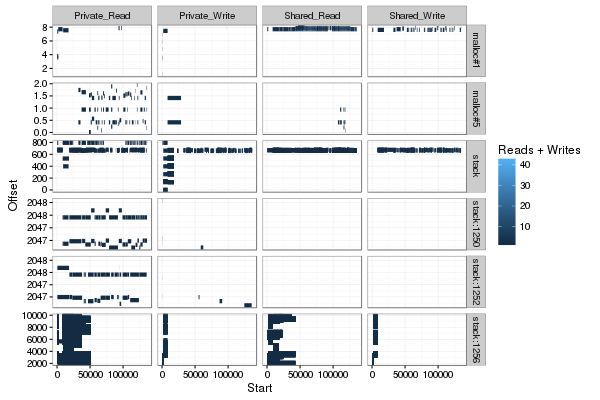
\includegraphics[width=\textwidth]{labbook/intensity_Rw_dgetrf}
    \caption{Visualization of the memory access of the dgetrf kernel from ffplas-ffpack.}
    \label{fig:dgetrf-intensity}
\end{figure}

We illustrate our visualization with the \emph{dgetrf} kernel from the fflas-ffpack~\cite{group16FFLASFFPACK} compiled against the OpenBlas~\cite{Chothia16OpenBlas}.
This trace was collected on a machine from the Edel cluster which hardware was presented in \tbl{hw-moca}.

\fig{dgetrf-intensity} shows for each data structures\footnote{
    A few almost unused data structures have been filtered out to make the image more readable.}
    the number of accesses per page over the time.
Furthermore we differentiate four types of access: \texttt{PrivateRead}, \texttt{PrivateWrites}, \texttt{SharedRead} and \texttt{SharedWrites}.

For each structures, some accesses seemed to appear private and shared at the same time which is not possible.
Nevertheless, by zooming on a small part of the execution were able to confirm that those access are interleaved and never of both types at the same time.
This means that several threads are working on data very close and often do actually share some pages.

From this visualization we can see that two of the stacks (1252 and 1250) are always used privately.
Furthermore the data structure malloc\#5 seems to be used mostly privately and only very rarely read in a shared way.
These three structures seems also to be accessed mostly linearly, hence they should not be subject to memory optimization.

\lstinputlisting[caption={R code to focus on interesting data structures.}, label=lst:R-zoom,float=htb]{code/zoom.R}

At this point, it is interesting to focus on these three data structures and ignore the others, we can do this with the simple line of code displayed in \lstr{R-zoom}.
Additionally, we can look at the amount of sharing instead of the number of axis just by changing the \emph{y} parameter of the plot.

\begin{figure}[htb]
    \centering
    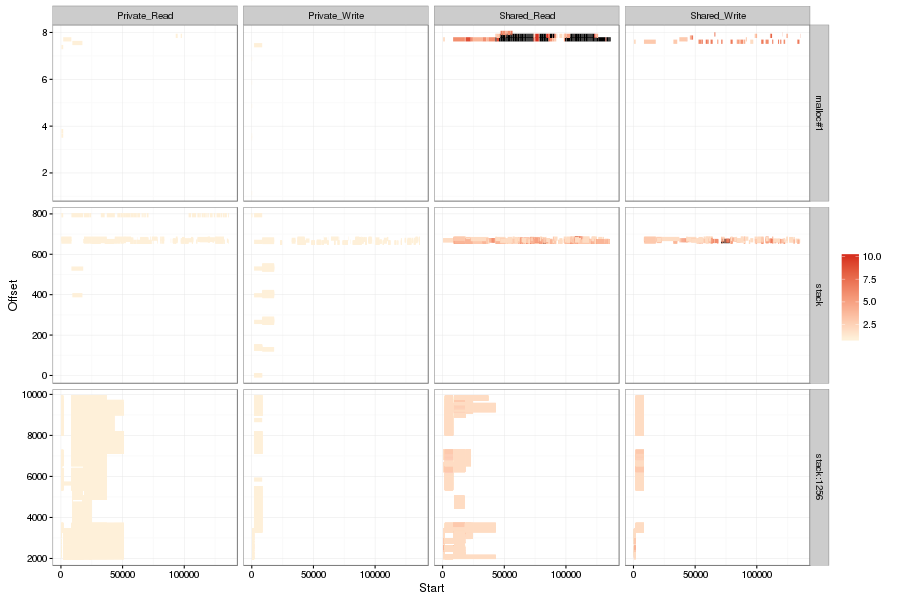
\includegraphics[width=\textwidth]{labbook/intensity_Share_dgetrf_zoom}
    \caption{Visualization of the memory access of the dgetrf kernel from ffplas-ffpack, zoom on the three interesting data structures.}
    \label{fig:dgetrf-share-zoom}
\end{figure}

We can see in \fig{dgetrf-share-zoom} that the sharing patterns are very similar to the access patterns.
The three other data structures present different and interesting memory access patterns.
First the malloc\#1 structure is very small and accessed intensively in a shared way, during all the execution and always on the same page.
We can presume that this data structure contains information about the threads status that must be updated quite often, maybe it is used for thread scheduling.
Second the stack 1256 is only used during the first third of the execution and written only at the beginning and in parallel.
For a generic data structure, this parallel initialization could probably have been designed to distribute first touch on the \gls{NUMA} nodes of the machine, still on a stack it seems quite unusual.
Last but not least, a small part of the main stack is accessed in read and write mode and in a shared way during all the execution.
This pattern means that threads are probably organized in a master / slave way, where the master thread allocates data in its stack (not dynamic allocation).
This might be problematic on \gls{NUMA} machines as the stack is statically allocated and thus cannot be allocated explicitly on some node.
It would be interesting to zoom on the beginning of the execution to check if the initialization of this part of the stack is correctly spread around the thread or not.
If not, Linux will allocate each page on the memory bank of the master thread independently of the re partition of the data between the threads.

After discussing these results with some of the developers of the fflas-ffpack, it appears that the observed patterns can be due to the OpenBlas library and might be complex to improve.
Yet an interesting thing to do would be to compare these traces, with the trace of the same kernel but compiled against the \gls{MKL}.
Indeed there are some performance differences between the two library that are hard to explain with traditional profiling tools as the \gls{MKL} code is proprietary.
Therefore, memory traces might help understanding the underlying algorithms.

In the end, this approach ease the exploration of \gls{Moca} traces, provided that we know a minimum of \gls{R} code.
Moreover, while \gls{Framesoc} and \gls{Ocelotl} can be easily used by an end user without the our intervention, at the time of the writing, this programmatic approach requires to read at least a part of the labbook to understand how to do the analysis.
Additionally, we had some troubles to analyze some traces from Lulesh \gls{OpenMP} and \gls{SOFA}.
Indeed these applications generates thousands of call to the malloc functions (hundreds of thousands for Lulesh).
Hence, retrieving the mapping page to data structure was extremely slow or nearly impossible without merging some data structures.
In the end it appears that we need both a more user friendly tool, and a way to add a priori knowledge of the developers in the parsing step to filter out uninteresting data.

\subsection{Generic trace visualization tool}

Programmatic exploration of traces is extremely powerful but not user friendly.
We describe here an hypothetical, generic trace viewer based on \gls{R} that should make trace exploration more user friendly.
We only provide some principles of design and interaction that results from our experiment while trying to analyze traces with \gls{R}.

\begin{figure}[htb]
    \centering
    %!TEX encoding=UTF-8 Unicode

% Layers
\pgfdeclarelayer{background}
\pgfdeclarelayer{foreground}
\pgfsetlayers{background,main,foreground}

\definecolor{TraceCol}{HTML}{B2ABD2}
\definecolor{UserCol}{HTML}{FDB863}
\definecolor{ViewerCol}{HTML}{E66101}
\definecolor{EntityCol}{HTML}{5E3C99}

\tikzstyle{entity} = [drawed box=EntityCol]
\tikzstyle{userbox} = [filled box=UserCol,shape=circle]

\tikzstyle{trace}  = [-latex,TraceCol,thick]
\tikzstyle{view} =   [-latex,ViewerCol,thick]

%\newlength{\cornerlength}
%\setlength{\cornerlength}{.1}

\tikzset{
  basic box/.style = {
    shape = rectangle,
    draw,
    text centered,
    text width=5em,
    },
  rounded box/.style={
    basic box,
    rounded corners,
  },
  drawed box/.style ={
    rounded box,
    draw = #1,},
  filled box/.style = {
    rounded box,
    draw  = #1,
    fill  = #1,
  },
  concrete box/.style = {
    shape = rectangle,
    text centered,
    text width=5em,
    draw  = #1,
    fill  = #1,
  },
    corner/.style={
      shape=rectangle,
      fill=white,
      alias=this,
      append after command = {
          \pgfextra{
              \begin{pgfonlayer}{foreground}
                % Borders of the corner
                \draw [] (this.south west) -- (this.south east);
                \draw [] (this.south west) -- (this.north west);
                \draw [] (this.north west) -- (this.south east);
                % Borders of the main rectangle
                \draw [] (#1.north west)   -- (this.north west);
                \draw [] (#1.north west)   -- (this.north west);
                \draw [] (#1.north west)   -- (#1.south west);
                \draw [] (#1.south west)   -- (#1.south east);
                \draw [] (#1.south east)   -- (this.south east);
              \end{pgfonlayer}
            }
      }
  },
  file/.style ={
      shape = rectangle,
      text centered,
      fill = TraceCol,
      minimum height = 5.5em,
      text width = 3.5em,
      append after command = {
            \pgfextra{\let\TikZlastnode\tikzlastnode}
                node [corner=\TikZlastnode, anchor=north east] (corner-\TikZlastnode) at
                (\TikZlastnode.north east){}
          }
  },
  fileT/.style ={
      file,
      fill =TraceCol,
  },
  fileV/.style ={
      file,
      fill =ViewerCol,
  },
  header node/.style = {
    %Minimum Width = header nodes,
    font          = \strut\large,%\ttfamily,
  %  text depth    = +0pt,
    fill          = #1,
    text         = white,
    draw},
    header/.style n args={4}{%
    inner ysep = +1.7em,
    append after command = {
      \pgfextra{\let\TikZlastnode\tikzlastnode}
      node [header node=#2,#4] (header-\TikZlastnode) at (\TikZlastnode.#3) {#1}
      %node %[span = (\TikZlastnode)(header-\TikZlastnode)]
       % at (fit bounding box) (h-\TikZlastnode) {}
    }
  },
  hv/.style = {to path = {-|(\tikztotarget)\tikztonodes}},
  vh/.style = {to path = {|-(\tikztotarget)\tikztonodes}},
  fat blue line/.style = {ultra thick, blue}
}
\begin{tikzpicture}[font=\small,scale=1]


    \node [userbox] (user) at (0,0) {User};

    \node[filled box=ViewerCol] (shell) at (3,0) {\textbf{Shell:} R and Commands (pop, zoom, filtrate)};

    \node[filled box=ViewerCol] (stack) at (5.5,0) {R dataframe Stack};

    \node [fileT] (f0) at (8,0) {Main Data};
    \node [fileT] (f1) at (10,0) {Meta Data};
    \node [fileT] (f2) at (9,-2.5) {Other File};

    \begin{pgfonlayer}{background}
        \node[entity,fit=(f0) (f1) (f2),%
        header={Trace}{EntityCol}{north}{}] (trace) {};
    \end{pgfonlayer}

    \node [filled box=TraceCol]   (rqf) at (6, -6) {Required files};
    \node [concrete box=TraceCol] (pc) at  (9, -6) {Parsing code};
    \node [concrete box=TraceCol] (pp) at  (7.5,-8) {Predefined plots};

    \begin{pgfonlayer}{background}
        \node[entity,fit=(rqf) (pc) (pp),%
        header={Configuration}{EntityCol}{south}{}] (config) {};
    \end{pgfonlayer}


    \begin{pgfonlayer}{background}
        \node[entity,draw=ViewerCol,fit=(shell) (stack),%
            header={Viewer}{ViewerCol}{north}{}] (viewer) {};
    \end{pgfonlayer}

    \path[trace]  (rqf.north) edge[out=90,in=-90] node[pos=.3,above] {Defines} (trace.south);

    \path[view] (viewer.south) edge[out=-90,in=180] node[pos=.3,right] {Loads} (config.west);

    \draw[view] ($(user.east)+(-.1,.2)$) -- ($(viewer.west)+(0,.2)$);
    \draw[view] ($(viewer.west)+(0,-.2)$) -- ($(user.east)+(-.1,.-.2)$);

\end{tikzpicture}
% vim: et si sta lbr  sw=4 ts=4 spelllang=en_us

    \caption{Description of a R based hypothetical generic trace viewer.}
    \label{fig:generic-viewer}
\end{figure}

The main components and interactions of our hypothetical tool are presented in \fig{generic-viewer}.
To be generic this tool is split in two parts: the viewer itself is quite minimalist, it contains a few predefined commands for interacting with data (zoom, filters \ldots), with the dataframe stack that will be described later and do predefined actions (parse, show some plot).
The second part is the configuration and should be provided by the developer of the tracing tool.
This configuration defines six things:
\begin{itemize}
    \item The code required to implement the trace interaction commands (zoom, filter etc.).
    \item Optionally some code to define some specific commands.
    \item The files that constitute the trace.
    \item The code used to do the parsing steps.
    \item Some breakpoints that can be used to insert code during parsing.
    \item The code used to provide the main predefined plots.
\end{itemize}

Another important idea is that the tool should conserve a \emph{dataframe stack} which means that the users will work on a small set of dataframes, and every modification to a dataframe (except if specified otherwise) should generate a copy.
While this means a considerable memory footprint, it enables rolling back if a step of aggregation (for instance) loose too much information.
Moreover, the first step of the analysis often consists in filtering data to focus on the most meaningful part of the trace.
Hence, only the first copies will have an important impact on the memory footprint.

The users would have two ways to interact with this tool: use builtin commands (or commands defined by the tool), or \gls{R} code.
These two usage are not incompatible.
At any step the users can see the code of the next step that they want to run and modify it or execute it.
A natural workflow would be to start analyzing the trace with the commands provided with the trace, and if necessary, start running \gls{R} code to generate new visualizations or filter data.
In the end, the user would be able to export the code of the new visualization to improve the original configuration.

\section{Discussions}
\label{sec:visu-cncl}

Visualizing \gls{Moca} traces is a complex task.
Indeed these traces are spread over five dimensions: time, addresses (virtual or physical), threads, \gls{CPU} location and access type.
Furthermore, the address space is quite large and we are mostly interest on some specific patterns.
Therefore, we first used \gls{Ocelotl} to analyze these traces.
This tool is designed to aggregate traces in a meaningful way, trying to provide a good trade-off between information lost and data reduction.
Moreover it is implemented as a \gls{Framesoc} tool.
\gls{Framesoc} is a generic trace manager, that provide a simple \gls{API} to import traces from virtually any tools.
Importing \gls{Moca} traces inside \gls{Framesoc} is also interesting as it provides easy filtering and zoom on the traces.
Still, \gls{Framesoc} considers that a trace has two dimensions: time and event producers, it is hard to represent the complexity of \gls{Moca} traces in it.
As a result, we had to generate several different \gls{Framesoc} traces while importing one \gls{Moca} trace.
The main drawback of this workaround is that switching traces inside \gls{Framesoc} means loosing all zooms and filters along with the caches and the results of the aggregated views computed by \gls{Ocelotl}.
In the end this approach enable the visualization of small traces, yet the cost of changing the perspective is too high and makes the interaction too slow to be usable.

Our second approach to analyze these trace was more programmatic, we use \gls{R} and saved all our attempts in a labbook.
While this is not user friendly at all, \gls{R} is a powerful tool and it enables more complex visualization.
We are able to do efficient and complex zoom with \gls{R} selection operators.
To make this analysis reproducible by users not familiar with \gls{R}, it would be interesting to develop a generic viewer build upon predefined \gls{R} visualization.
Such viewer should (at least) provide the two following feature: simple (non \gls{R}) zoom and filtering and a dataframe stack so the users can rollback if they discard some useful informations.

Another approach that have not been studied during this thesis would be to analyze traces automatically.
Such analysis would have to detect memory patterns and possibly and highlight parts of code that should be improved.
A memory pattern is an interaction between threads inside a memory area over a short laps of time.
Yet, defining such a pattern in a more specific way is a hard task.

For any approach, it appears that the developers knowledge is useful to focus the analysis on the interesting parts.
Therefore we need a way to use this knowledge during the analysis and as soon as possible to reduce the amount of data we need to analyze.
Nerveless, we have seen in \chap{perf} that they might not know all the source of performance issues.
In the end, this knowledge can be used to focus the analysis but it is important to also have a global visualization of the trace, to spot issue that would have been missed by the developers.
Hence the two approaches described in this chapter can be used in a complementary way.

% vim: et si sta lbr  sw=4 ts=4 spelllang=en_us
